% \textbf{Title: Integral Calculus 4}

The graph of \( f(x) \) is given.

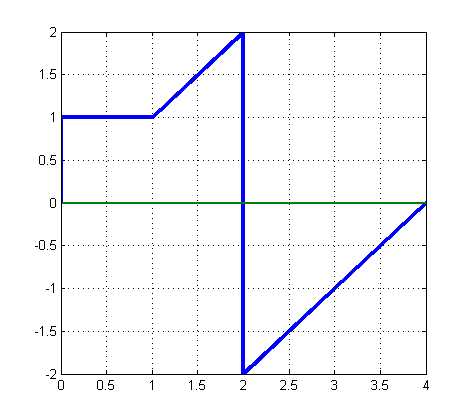
\includegraphics[width=1.71005in,height=1.52489in]{../../Images/IntegralCalculusQ1234.png} 

How should \(a\) and \(b\) be chosen so that \( \int_a^b f ( x )\ dx = 0 \) ?\\


a. \( ( a,\ b ) = ( 0,\ 4 ) \)

*b. \( ( a,\ b ) = ( 1,\ 3 ) \)

c. \( ( a,\ b ) = ( 0,\ 2 ) \)

d. \( ( a,\ b ) = ( 2,\ 4 ) \)

e. I do not know.\\
